\documentclass[a4paper,english]{article}
\usepackage{indentfirst}
\usepackage{graphicx}
\usepackage{epstopdf}
\usepackage{amssymb}
\usepackage{amsmath}
\usepackage{latexsym}
\usepackage{fancyhdr}

\usepackage{subfigure}
\usepackage{epstopdf,color}

%\usepackage[CJKbookmarks,pdfpagemode=UseOutlines,bookmarksnumbered,bookmarksopen]{hyperref}
%\hypersetup{CJKbookmarks,bookmarksnumbered,colorlinks,linkcolor=black,citecolor=black,plainpages=false,pdfstartview=FitH}
\usepackage{longtable}
\usepackage{booktabs}
\usepackage{bm}
\usepackage{type1cm}
\usepackage{xcolor}
\usepackage{pifont}
\usepackage{titlesec}
\usepackage{float}
\usepackage{comment}
\usepackage{mathrsfs}
\usepackage{graphicx}
\setlength{\textwidth}{6.5in}
\setlength{\oddsidemargin}{0in}
\setlength{\evensidemargin}{0in}
\setlength{\topmargin}{0.20in}
\setlength{\textheight}{8.8in}
\setlength{\footskip}{0.6in}
\setlength{\headsep}{0in}

\usepackage[utf8]{inputenc}
\usepackage{natbib}
\usepackage{graphicx}
\usepackage{subfigure}
\usepackage{amssymb}
\usepackage{amsmath}
\usepackage{amsthm}
\usepackage{mathtools}
\usepackage{mathrsfs}
\usepackage{epstopdf}
\usepackage{booktabs}
\usepackage{setspace}
\usepackage{cases}
\usepackage{dsfont}
\usepackage[colorlinks,linkcolor=blue,anchorcolor=blue,citecolor=blue,urlcolor=blue]{hyperref}
\usepackage{algorithm}
\usepackage[noend]{algpseudocode}

\usepackage{tikz}
\usepackage{forest}

\newtheorem{col}{Corollary}[section]

\renewcommand{\baselinestretch}{1.5}
\newcommand{\book}[1]{\textit{#1}}
\newcommand{\C}{\textbf{Comments:}}
\newcommand{\Q}{\textbf{Questions:}}
\newcommand{\pth}[1]{\left( #1 \right)}
\newcommand{\br}[1]{\left[ #1 \right]}
\newcommand{\cur}[1]{\left \{  #1 \right \}}
\newcommand{\vct}[1]{\boldsymbol{#1}}
\newcommand{\mat}[1]{\boldsymbol{#1}}
\newcommand{\abs}[1]{| #1 |}
\newcommand{\norm}[1]{|| #1 ||}
\newcommand{\set}[1]{\left \{  #1 \right \}}
\newcommand{\mon}[1]{\left \langle #1 \right \rangle}
\newcommand{\Rset}{\mathbb{R}}
\newcommand{\pt}[1]{\dot{#1}}

%\usepackage{geometry}
%\geometry{left=4cm,right=4cm,top=3cm,bottom=3cm}
\usepackage{ulem}
\usepackage{CJK}
\usepackage{setspace}
\usepackage{amsthm}
\usepackage{abstract}
\usepackage{listings}
\usepackage{nameref}
\usepackage{graphicx}
\usepackage{color} %red, green, blue, yellow, cyan, magenta, black, white
\definecolor{mygreen}{RGB}{28,172,0} % color values Red, Green, Blue
\definecolor{mylilas}{RGB}{170,55,241}
%\renewcommand{\absnamepos}{flushleft}
\title{Analysis on the Binary Game}
\date{}
\author{Yixiang Luo, Qi Huang, Yahui Cui\footnote{This is a group project of Foundamental Algorithm class with Prof. Joel Spencer at New York University.}}
%\usepackage{ccmap}
%\hypersetup{CJKbookmarks=true}


\newtheorem{example}{Ex}[section]
\newtheorem{defn}{Def}[section]
\newtheorem{thm}{Theorem}[section]
\newtheorem{rem}{Rmk}[section]
\newtheorem{lem}{Lemma}[section]

\begin{document}
\maketitle
\begin{spacing}{1.4}


\begin{abstract}
We analyze the evolution of the value of the ``binary game'' from both numerical and analytical perspective. We find numerically that the game value oscillate around zero and seems to have two converged subsequences, which indicates a stable advantage to playing last. Moreover, the empirical variance of the game value also converge to zero. In theoretical analysis, we prove all these observations and find the limits as $n \to \infty$ as an even or odd number sequence. The limits are related to the golden ratio, i.e. $(\sqrt{5}-1)/2$, which is quite beautiful.
\end{abstract}

\section{Introduction}
In this project, we are to analyze the value of a sequential zero sum game, which we called Binary Game. The game has $n$ moves, alternating between Paul (first) and Carole. At each move the player selects a bit, zero or one. The starting node, denoted $e$, is the empty string. After $u$ moves the intermediate node will be a binary string of length $u$. At the end of the game, the leaves are the $2^n$ strings of length $n$. The values $VALUE(x)$ for the leaves $x$ are set in advance. In particular it obeys the uniform distribution on $[-1,1]$. Paul wants to maximize the value while Carole wants to minimize it. When both of them take their optimal strategy, the value of the game is difined as the value of the root node, i.e. $VALUE(e)$. Our goal is to analyze the value of the game as $n$ increase. Detailed information about the game can be found in \cite{SpencerGame}.

A typical structure of the game looks like the follows.
\begin{center}
  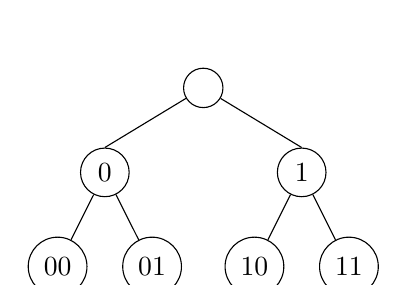
\begin{tikzpicture}[
    node/.style={circle, draw, rounded corners=1mm, text centered, anchor=north, text=black, minimum size=5mm},
    empty/.style={circle, draw=none, text centered, anchor=north, text=black, size=5mm},
    level distance=0.5cm,
    growth parent anchor=south,
    ]
      \node [node] {$~$}
      [sibling distance=2.5cm]
      child{ [sibling distance=1.2cm]
        node [node] (a) {$0$}
        child{
          node [node] {$00$}
        }
        child{
          node [node] {$01$}
        }
      }
      child{ [sibling distance=1.2cm]
        node [node] (a) {$1$}
        child{
          node [node] {$10$}
        }
        child{
          node [node] {$11$}
        }
      };
  \end{tikzpicture}
\end{center}

\section{Algorithm and implementation}
We follow the DFS algorithm described in \cite{SpencerGame} and Algorithm \ref{algo-game} shows the pseudocode for the core algorithm.

\begin{algorithm}
\caption{Binary Game’s algorithm (an Algorithm of Depth First Search)} \label{algo-game}
D is the distribution from which leaf values are sampled.
\begin{algorithmic}[1]
\Procedure{Game Value}{$P,H$}\Comment{P is position, H is player}
\If{$P=ROOT$}
\State $H\gets Player1$
\Else
\State $Pass$
\EndIf
\If{$P=LEAF$}
\State $Value\gets x \sim D$
\State \textbf{return} $Value$
\Else
\If{$F=Player1$}
\State $Value \gets \max\limits_{ i \in Adj[P]}\{Game Value(i,Player2)\}$ \Comment{Max Strategy}
\State \textbf{return} $Value$
\Else
\State $Value \gets \min\limits_{ i \in Adj[P]}\{Game Value(i,Player1)\}$ \Comment {Min Strategy}
\State \textbf{return} $Value$
\EndIf
\EndIf
\EndProcedure
\end{algorithmic}
\end{algorithm}

The implementation is a little bit tricky. The code with comments can be found in attached python files and we simply describe the implementation here for reference.

we define several classes to facilitate us implementing this algorithm.
\begin{enumerate}
  \item The tree class. It represents the tree of all possible "board situations" of this binary game, with depth $n$ as game's total unrolled steps, within which contains a nested Position class and a Node Class.
  \item The position class. This is an abstraction of a specific, i.e. current position in the whole course of this binary game.
  \item The node class. This class is not exposed to the user and stores actual information of a specific position, i.e. position's value, its parent position as well as its child position.
\end{enumerate}

We initialize a game by recursively calling \textit{gen\_board} function, which sample the leaves' initialized values from a given distribution. After initializing the game, we scores it by recursively calling two functions, \textit{scoring\_max\_min\_first} and \textit{scoring\_max\_min\_second}. The visualization codes naturally follows.

\section{Numerical results}
\subsection{Trend of the game value: oscillation and convergence of variance}
We conducted 500 times experiments for each $n \in [1,20]$, computed and plotted the mean and variance of the game value for each $n$, where $n$ is the total steps of our game.

\begin{figure}[htb!]
\centering
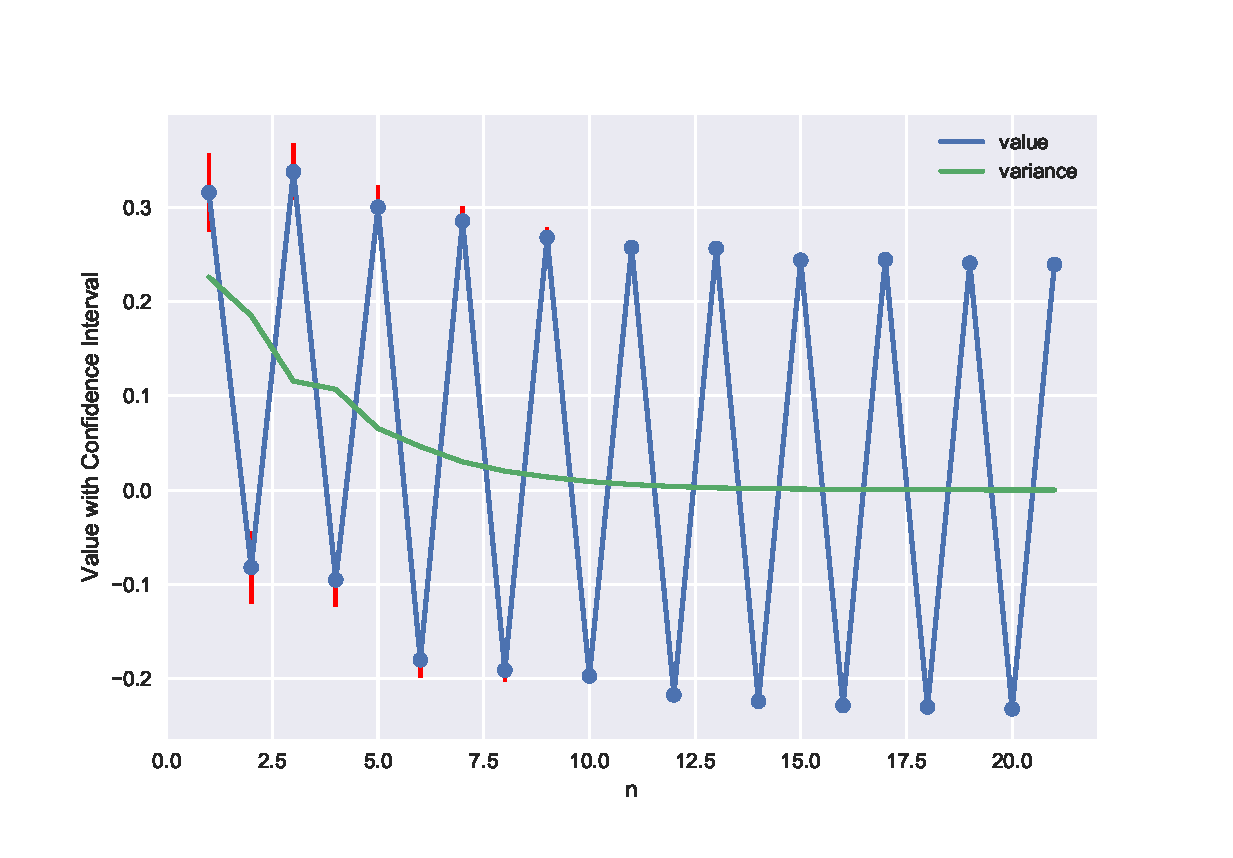
\includegraphics[width=0.8\textwidth]{figures/plot1.eps}
\caption{Value trend: oscillation and convergence of variance}
\label{oscillate}
\end{figure}

\paragraph{Value trend: oscillation}
By taking a look at the original data, we first noticed the relationship between $n$ and the mean value. In Figure \ref{oscillate}, we found the mean of game value fluctuates in a zigzag version with the increasing of $n$. Because Paul always play at first, the game value goes down from $n=1$ to $n=2$. Assuming we are at $n=i$, if mean value goes up from $i-1$ to $i$, then it goes down from $i$ to $i+1$ and vice versa. If we looked at the range of value and the corresponding $n$ more precisely, we found that with $n$ increasing, the mean of value fluctuates in a constant range, changing between positive and negative. When $n$ is odd, the mean value is always positive and goes to negative in the next time; if n is even, the value is negative and will become positive later. Besides, the mean never goes to zero, indicating there is advantage in this game.
\paragraph{Value trend: convergence of variance}
Our next observation focused on the variance of experiments for each $n$. With the same sample number for every $n$, however, we found the variance of the sampled game value decreasing rapidly with the increasing of $n$. It starts from around 0.25 and converges to 0. The convergence of sample variance has no relationship with the parity of $n$.
\paragraph{Summary: advantage, variance and two converged sequences}
Our observations on mean and variance of the sampled game value motivated us to search the game value in the way below:
\begin{enumerate}
    \item The relationship between parity of $n$ and the mean of game value suggests us to study the trend in two cases separately, when $n$ is even and odd. This is reasonable as we know when $n$ is odd, Paul will play the last step and has control of the final result by choosing the maximum value of all leaves; while when $n$ is even, Carol will play the last step by choosing the minimal value of all leaves and the only thing for Paul is to receive the game result. That is to say, the advantage comes in the last step.
    \item The change of variance is a little bit amazing to us, which implies that in either case, the game value may converge with the increasing of $n$, regardless to the parity of $n$.
    \item Together with the two points above, we infer that the game value might converge to two different points when $n$ goes to infinity and the points depend on the parity of $n$.
\end{enumerate}

\subsection{Distribution of game value}

\paragraph{Convergence to different points}
The game value converges when $n$ goes to infinity, but the points converged to are different when $n$ is odd or even.
We plotted the histograms of the sampled game value in two groups and normed the graph so that the sum of the area of each bin is 1. The x-axis is the value, while y-axis denotes the probability density of the corresponding score. We denote $(a_i,b_i)$ is the $i_{th}$ bin of the histogram, $N_i$ is the number of sample in that bin and $N$ is the number of samples for each $n$ and normed the graph in the way below, where $p(value=X)$ is the probability density of value when $value = X$:
\begin{equation*}
    P(X \in (a_i,b_i)) = \frac{N_i}{N}
\end{equation*}
\begin{equation*}
    p(value = X, X \in (a_i,b_i)) = \frac{P(X \in (a_i,b_i))}{(b_i,a_i)}
\end{equation*}
Figure \ref{distribution-odd} shows the odd case of $n$ with $n=15,17,19,21$. We observed that the distribution of sampled game value in each subplot forms a normal distribution asymptotically, centering around the mean of that sample. When $n$ increases, the distribution shrinks to the corresponding center, which verifies the decreasing variance when $n$ increases. The center for each distribution, however, also converges to some point between $(0.20,0.30)$.
\begin{figure}[htb!] \label{distribution-odd}
\centering
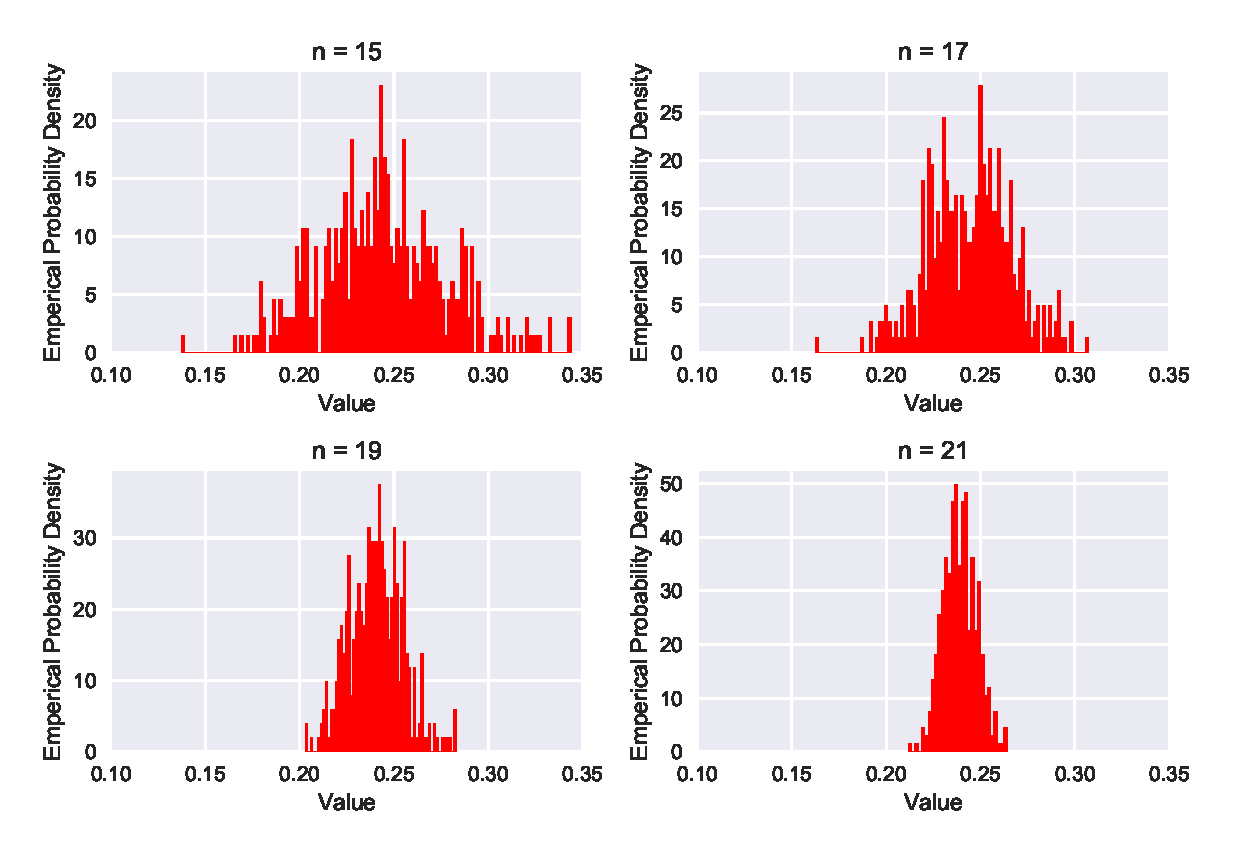
\includegraphics[width=0.8\textwidth]{figures/plot2.eps}
\caption{Game Value Distribution: $n$ is odd}
\end{figure}
Figure \ref{distribution-even} represents the case when $n$ is even, where $n = 14, 16, 18, 20$. The change of the distribution is similar to the case when $n$ is odd except that the center for each distribution converges to some point in $(-0.25, -0.15)$.
\begin{figure}[htb!] \label{distribution-even}
\centering
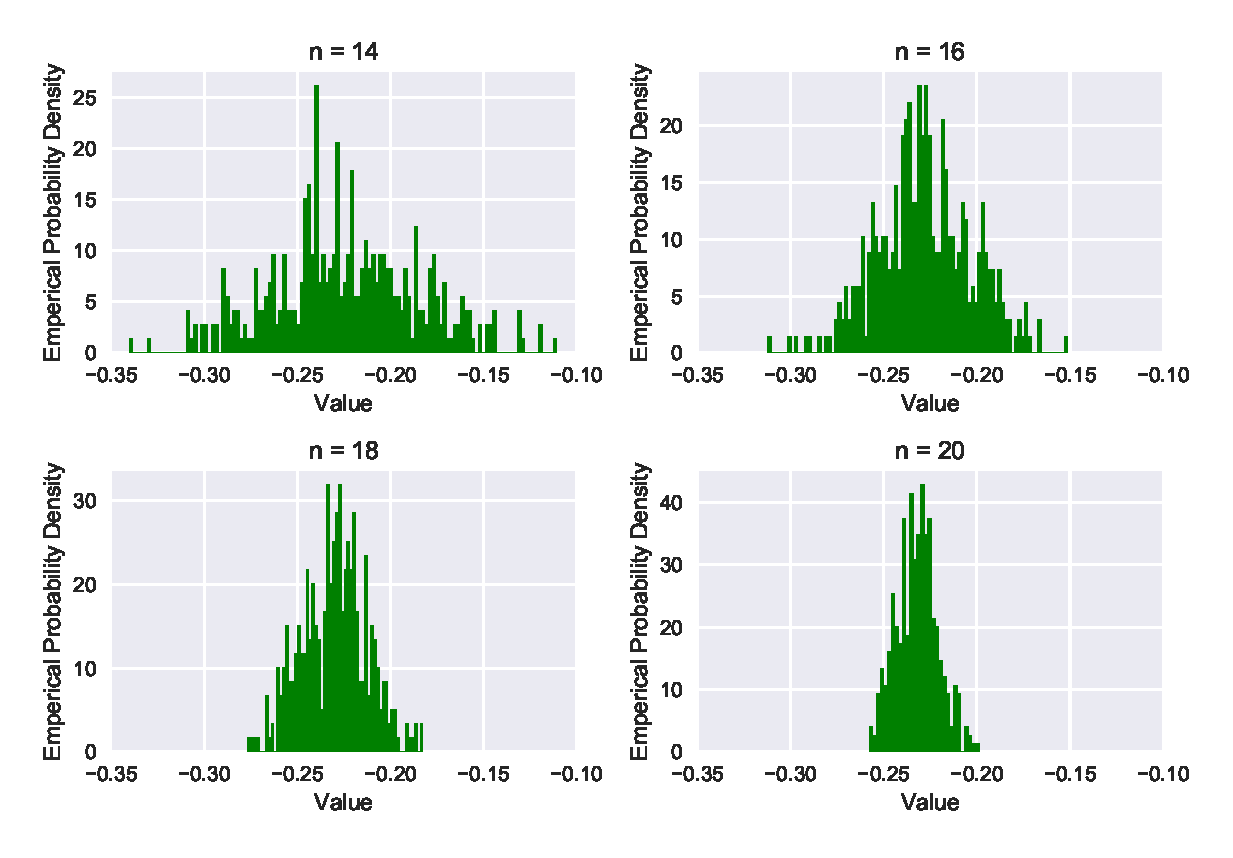
\includegraphics[width=0.8\textwidth]{figures/plot3.eps}
\caption{Game Value Distribution: $n$ is even}
\end{figure}
\paragraph{Density of the converged points (limits)}
The probability density of the converged points, which are limits, goes to infinity with $n$ going to infinity.
Figure \ref{game-value-pdf} shows a more clear trend for the distribution of game value under different $n$. With y-axis representing the probability density estimated from the histograms, all red lines denote the game value distribution when $n$ is odd, while all green lines represent that when $n$ is even. For all the red lines, we could see while the center of each distribution converges to one point in $(0.20,0.30)$, the peak of each distribution increases rapidly. This implies that the density of the center increases quickly with the increasing of $n$. Denote the point which the game value converges to as $X_{odd}$ and $X_{even}$ when when $n$ is odd and even respectively, the trend also suggests that the probability density of $X_{odd}$ goes to infinity. The trend for distribution of game value when $n$ is even is rather similar. With the center of all distribution converges to a point $X_{even}$ in $(-0.25, -0.15)$, the peak of the distribution increases fast and goes to infinity.
\begin{figure}[htb!] \label{game-value-pdf}
\centering
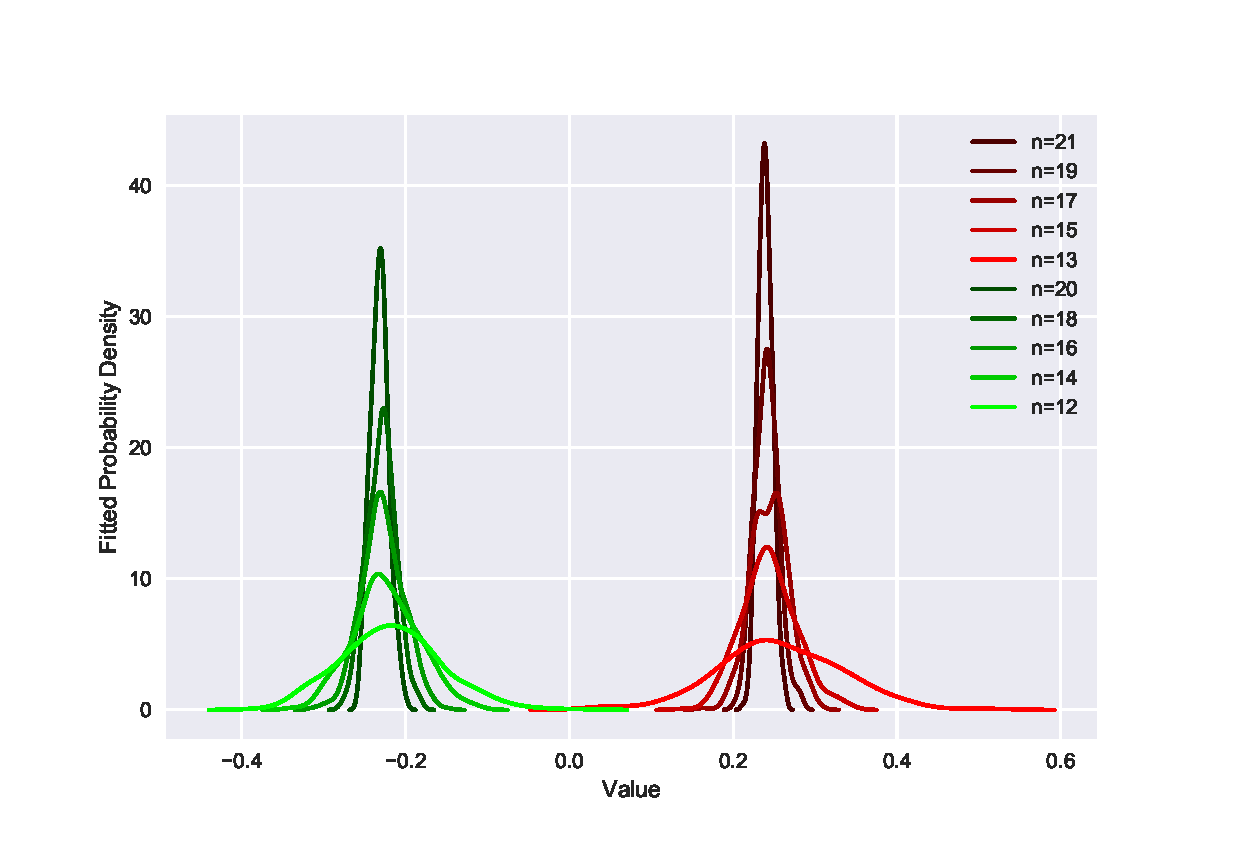
\includegraphics[width=0.8\textwidth]{figures/plot4.eps}
\caption{Game value distribution and fitted probability density}
\end{figure}

\subsection{Properties of the limits (converged points)}
\paragraph{Estimation of limits}
Besides the convergence, we also want to find some properties of the two limits, $X_{odd}$ and $X_{even}$. We first estimated the value of limits with n in different parity by choosing corresponding point of the maximum estimated density. Figure \ref{pdf-odd} and Figure \ref{pdf-even}. present our estimated probability density for the middle point of each bin with $n$ in odd and even, respectively. Table \ref{Game-value-table} shows our estimation of the limits for each $n$.
\begin{figure}[htb!] \label{pdf-odd}
\centering
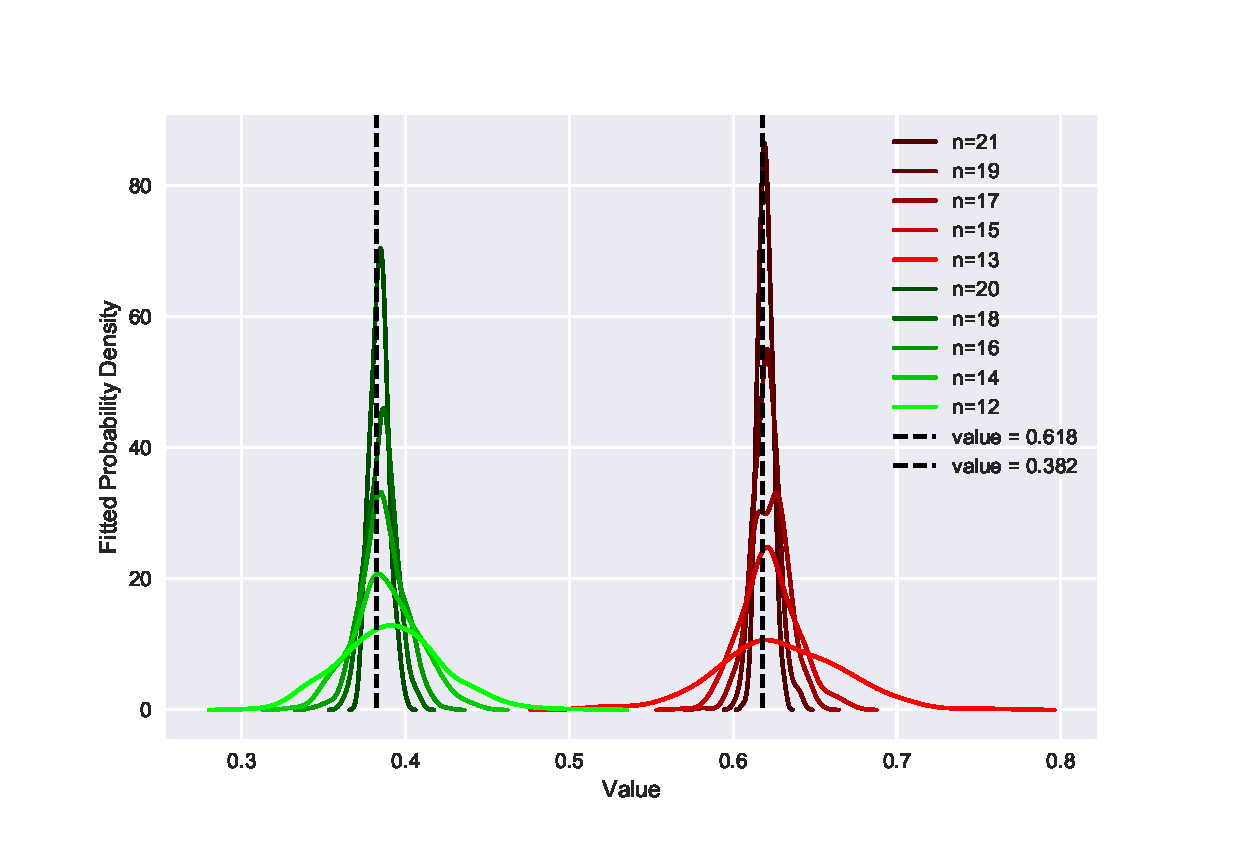
\includegraphics[width=0.8\textwidth]{figures/plot5.eps}
\caption{Estimated probability density:  $n$ is odd}
\end{figure}

\paragraph{Relative position to value range}
\begin{figure}[htb!] \label{pdf-even}
\centering
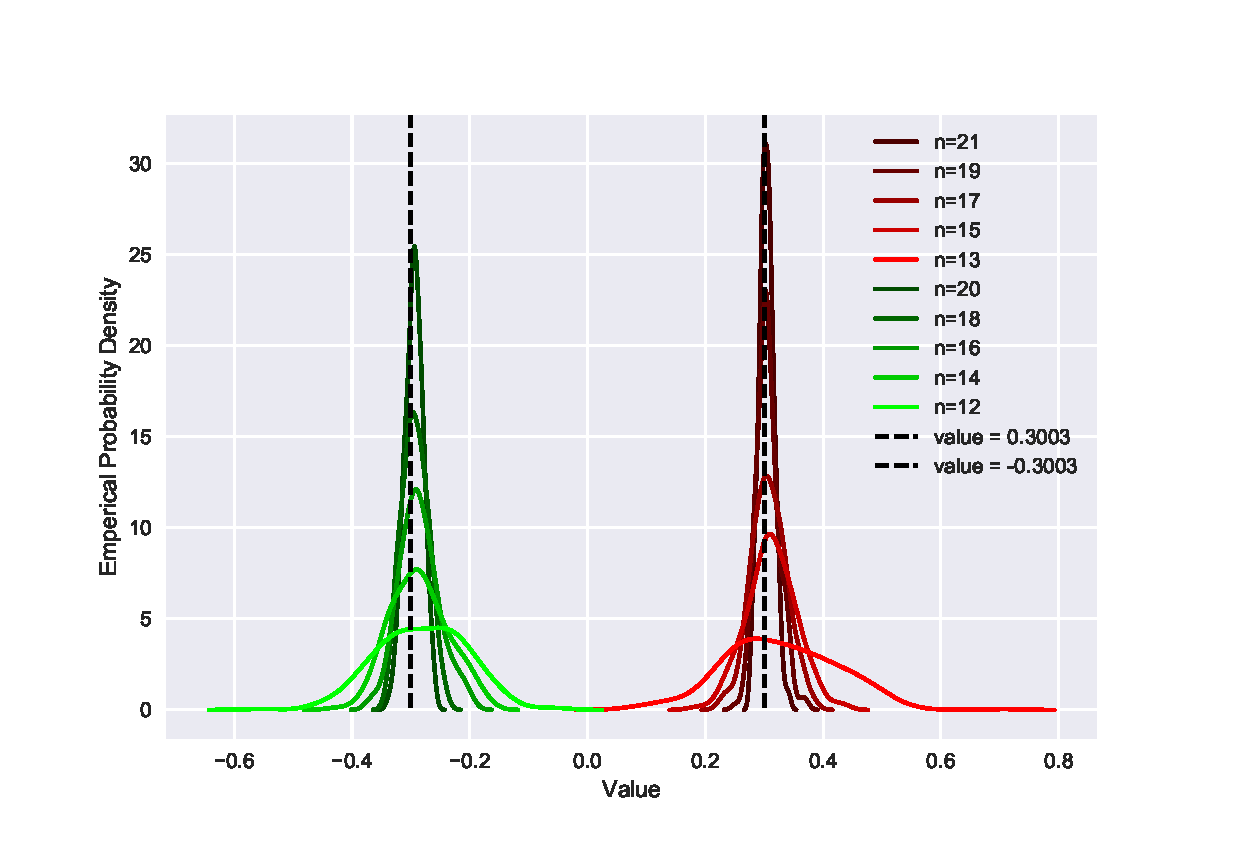
\includegraphics[width=0.8\textwidth]{figures/plot6.eps}
\caption{Estimated probability density:  $n$ is even}
\end{figure}

\begin{table} \label{Game-value-table}
\centering
\begin{tabular}{lllll}
\hline
 $n$ & 15 & 17 & 19 & 21 \\
 \hline
 $X_{odd}$ & 0.2509 & 0.2564 & 0.2389 & 0.2353 \\
 \hline
 $n$ & 14 & 16 & 18 & 20 \\
 \hline
 $X_{even}$ & -0.2369 &  -0.2237 & -0.2249 & -0.2312 \\
 \hline
\end{tabular}
\caption{Game values on $X_{odd}$ and $X_{even}$}
\end{table}
\paragraph{Relative position to value range}
We also searched the relative position of the game value to the range of the game value. We denote $d_{odd}$ to be the relative position of $X_{odd}$, $d_{even}$ to be the relative position of $X_{even}$, $[a,b]$ to be the range of the game value, $M$ to be the middle of the range and $r$ to be the ratio of $|X_{odd}-M|$ and $|X_{even}-M|$. We define $d_{odd}$, $d_{even}$ and $r$:
\begin{equation*}
    d_{odd}=\frac{|X_{odd}-a|}{|b-a|} \quad d_{even}=\frac{|X_{even}-a|}{|b-a|}
\end{equation*}

\begin{equation*}
    r = \frac{|X_{odd}-M|}{|X_{even}-M|}
\end{equation*}

%%somthing new
Table \ref{relative-position} presents the relative positions of limits.

\begin{table} \label{relative-position}
\centering
\begin{tabular}{lllll}
\hline
 $n$ & 15 & 17 & 19 & 21 \\
 \hline
 $d_{odd}$ & 0.6254 & 0.6282 & 0.6194 & 0.6177 \\
 \hline
 $n$ & 14 & 16 & 18 & 20 \\
 \hline
 $d_{even}$ & 0.3816 &  0.3882 & 0.3876 & 0.3844 \\
 \hline
\end{tabular}
\caption{Relative position of $X_{odd}$ and $X_{even}$}
\end{table}

\paragraph{Summary of properties}
Combining Table \ref{Game-value-table} and Table \ref{relative-position}, we found the relative position of the limits is near to 0.38 when $n$ is odd while near to 0.62 when $n$ is even. Besides, the points to the middle of the range is nearly same, implying the ratio $r$ defined above is near to 1.

\section{Theoretical analysis}
Inspired by the numerical results, we further investigate the problem from the theoretical perspective. In this section, we prove that the game value converges for even or odd sequence of $n$ respectively and further find the limits.

\subsection{recurrence relation}

Let's start with recurrence relation between the node values. As defined in the game, each node has a value and it is a random variable. It is easy to show that if the values of all leaf nodes are i.i.d., the values of nodes having the same height are also i.i.d. Assume the leaf nodes have height $0$ and denote the cumulative distribution function (CDF) of the values on nodes having height $i$ as $F_i(x)$, and the corresponding random variable as $V_i$. In the algorithm, the value of a internal node is calculated by taking the maximum or minimum of its two children. So we have
\begin{equation}
  \left\{
  \begin{array}{ll}
    F_{i+1} = F_i^2, & \text{ if take maximum}\\
    F_{i+1} = 1 - (1 - F_i)^2 = 2 F_i - F_i^2, & \text{ if take minimum}
  \end{array}\right.
\end{equation}
Combining the order of playing of the game, we conclude that
\begin{equation}
  \left\{
  \begin{array}{ll}
    F_{i+1} = F_i^2, & \text{ if $i+n$ odd, $i \leq n-1$}\\
    F_{i+1} = 1 - (1 - F_i)^2 = F_i (2 - F_i), & \text{ if $i+n$ even, $i \leq n-1$}
  \end{array}\right.
\end{equation}

\subsection{convergence}
Now let's combine two successive updates and derive the relationship as follows.
\begin{numcases}{}
  F_{i+2} = L(F_i) \equiv F_i^2 (2 - F_i)^2, & \text{ if $i+n$ even, $i \leq n-2$} \label{two_step} \\
  F_{1} = F_0^2, & \text{ if $n$ odd} \label{init_ts}
\end{numcases}
What we concern about is the value of the root node, i.e. $F_n$. And the reccurence above is enough for this purpose. If $n$ is even, we apply (\ref{two_step}) on $F_0$ and finally we will reach $F_n$. If $n$ is odd, we apply (\ref{init_ts}) on $F_0$ and then (\ref{two_step}) and finally we will also reach $F_n$.

Now we can state our main result.

\begin{thm} \label{convergence}
The CDF of the value of the root node, i.e. $F_n$, converges pointwisely for even $n$ or odd $n$ sequence. Specifically,
\begin{enumerate}
  \item for even $n$, $F_n$ converge to $\mathds{1}_{x \geq x_1}$, where $x_1$ is the solution to $F_0(x_1) = 1 - \phi$;
  \item for odd $n$, $F_n$ converge to $\mathds{1}_{x \geq x_2}$, where $x_2$ is the solution to $F_1(x_2) = F_0^2(x_2) = 1 - \phi$, or equivalently, $F_0(x_2) = \phi$;
\end{enumerate}
where $\mathds{1}$ is the indicator function and $\phi = \frac{\sqrt{5}-1}{2}$ is the Golden ratio.
\end{thm}

\begin{proof}
  \begin{enumerate}
    \item Since $n$ is an even number, after applying $n/2$ times of reccurence (\ref{two_step}) on $F_0$ we get $F_n$. Now let's look at the difference after one reccurence
    \begin{equation}
      D(F_i) = F_{i+2} - F_i = L(F_i) - F_i = F_i^2 (2 - F_i)^2 - F_i
    \end{equation}
    For simplicity, let's ignore the subscript and simply write
    \begin{equation}
      D(F) = F^2 (2 - F)^2 - F.
    \end{equation}
    The function $D(F)$ has only three zeros in $[0, 1]$, which are
    \begin{equation}
      0, \quad 1 - \phi, \quad 1,
    \end{equation}
    and its graph is shown in Figure \ref{D_F}.
    \begin{figure}[!htb] \centering
      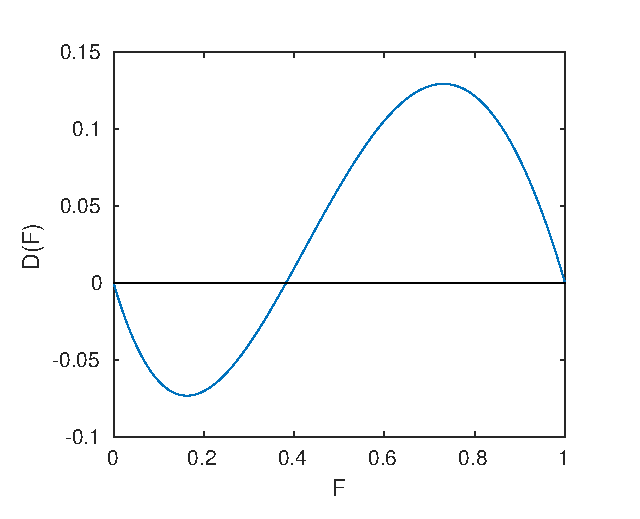
\includegraphics[width=0.4\columnwidth]{figures/D_F.eps}
      \caption{The graph of $D(F)$.}
      \label{D_F}
    \end{figure}

    If $F > 1 - \phi$, after applying the operator $L$ on F, $L(F) > F > 1 - \phi$. So $L^k (F)$ is a strictly increasing function of $k$, if $F > 1 - \phi$, where $L^k (F)$ means applying the operator $L$ $k$ time. In addition, since $L^k (F)$ is a restriction of the CDF $F_{2k}$, we have $L^k (F) \leq 1$. Therefore $F_{2k}(x) \; (F_0(x) > 1 - \phi)$ converges as $k$ goes to infinity.
    Moreover, since there is only one zero of $D(F)$ in $(1 - \phi, 1]$, which is $1$, the only stationary point of $L(F)$ in $(1 - \phi, 1]$ is $1$. Thus $F_{2k}(x) \; (F_0(x) > 1 - \phi)$ converges to $1$.

    Similarly, we have $F_{2k}(x) \; (F_0(x) < 1 - \phi)$ converges to $0$.

    Combining all above, we conclude
    \begin{equation}
      F_n(x) \to \mathds{1}_{F_0(x) \geq 1 - \phi}, \text{ as } n \to \infty, \quad \text{$n$ even}
    \end{equation}

    \item When $n$ is odd, applying the same analysis, but notice now the initial value of the reccurence (\ref{two_step}) is $F_1$ and $\sqrt{1-\phi} = \phi$, we derive
    \begin{equation}
      F_n(x) \to \mathds{1}_{F_1(x) \geq 1 - \phi} \equiv \mathds{1}_{F_0^2(x) \geq 1 - \phi} \equiv \mathds{1}_{F_0(x) \geq \phi}, \text{ as } n \to \infty, \quad \text{$n$ odd}
    \end{equation}

  \end{enumerate}
\end{proof}

Then we have the following corollaries immediately.
\begin{col}
  Denote the probability distribution function corresponding to $F_n(x)$ as $f_n(x)$. Then
  \begin{enumerate}
    \item for even $n$, $f_n$ converge to $\delta(x - x_1)$, where $F_0(x_1) = 1 - \phi$;
    \item for odd $n$, $F_n$ converge to $\delta(x - x_2)$, where $F_0(x_2) = \phi$;
  \end{enumerate}
  where $\delta(x)$ is the Dirac delta function.
\end{col}

\begin{col} Denote $\mathbb{E} (V_n)$ and $var(V_n)$ as the expectation and variance of $V_n$ respectively.
  \begin{enumerate}
    \item For even $n$, $\mathbb{E} (V_n) \to x_1$ and $var(V_n) \to 0$, where $F_0(x_1) = 1 - \phi$.
    \item For odd $n$, $\mathbb{E} (V_n) \to x_2$ and $var(V_n) \to 0$, where $F_0(x_2) = \phi$.
  \end{enumerate}
\end{col}

\begin{col}
  If the PDF corresponding to $F_0$ is even, then $x_1 = -x_2$, where $x_1, x_2$ defined as above.
\end{col}

\subsection{uniform distribution}
Assume $V_0 \sim U([-1, 1])$, which is the setting in this game problem. Now $F_0(x) = (x+1)/2$ and $F_1(x) = (x+1)^2/4$ (if $n$ odd). So
\begin{equation}
  x_1 = 1 - 2\phi, \quad x_2 = 2\phi - 1
\end{equation}
and
\begin{enumerate}
  \item For even $n$, $\mathbb{E} (V_n) \to 1 - 2\phi \approx -0.236$ and $var(V_n) \to 0$,
  \item For odd $n$, $\mathbb{E} (V_n) \to 2\phi - 1 \approx 0.236$ and $var(V_n) \to 0$,
\end{enumerate}
which is consistent with the numerical results.

As we can see in Figure \ref{Comparison}, the theoretical and numerical results are consistent. The black lines mark the limit distribution and red lines(odd case) and green lines(even case) are the empirical distributions.
\begin{figure}[htb!] \label{Comparison}
\centering
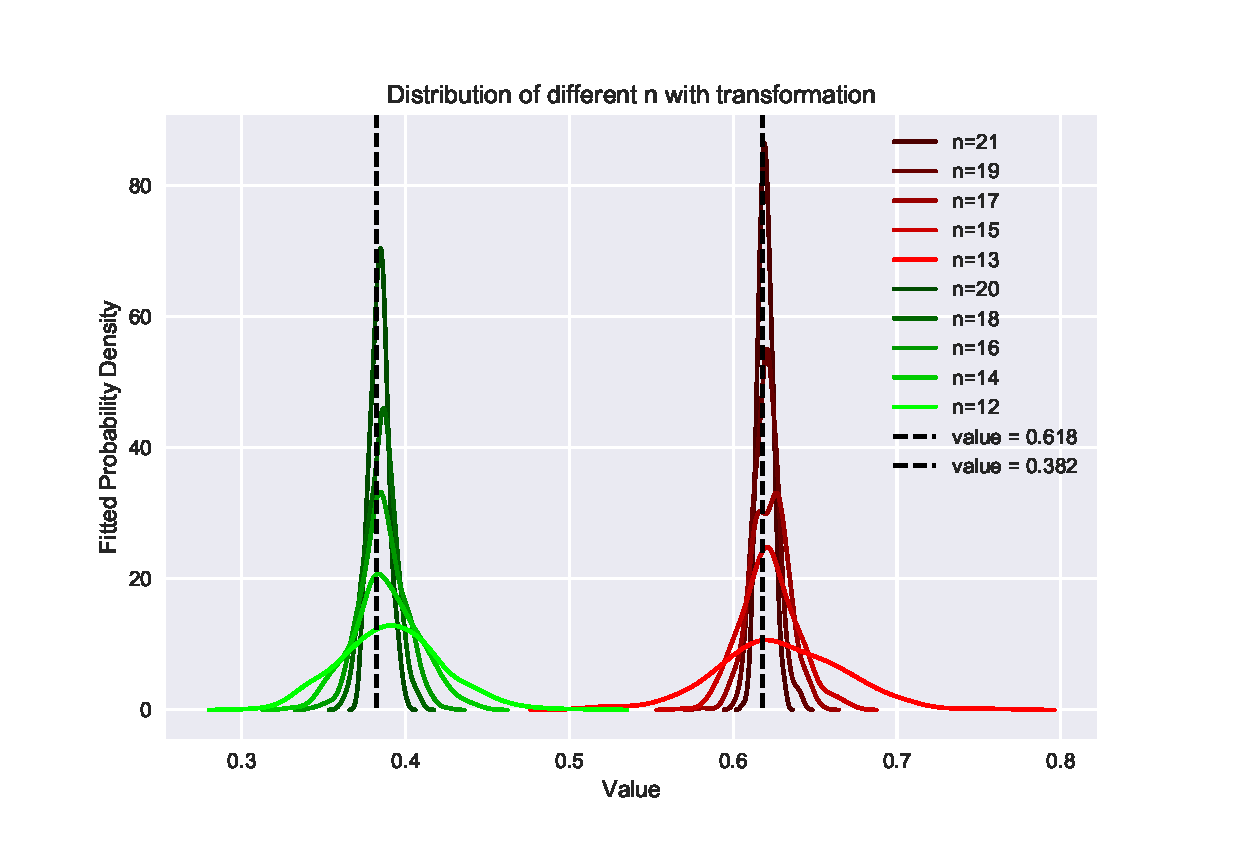
\includegraphics[width=0.8\textwidth]{figures/plot7.eps}
\caption{Comparison between theoretical distribution and experiment results}
\end{figure}

\section{Gaussian distribution}
For the Gaussian distribution $V_0 \sim \mathcal{N}(0, 1)$, we get
\begin{equation*}
  F_0(x) = \frac 12 \pth{1+erf(\frac{x}{\sqrt{2}})}, \quad F_1(x) = \frac 14 \pth{1+erf(\frac{x}{\sqrt{2}})}^2 \text{ (if $n$ odd)}
\end{equation*}
where
\begin{equation*}
  erf(x) = \frac{2}{\sqrt{\pi}} \int_0^x e^{-t^2} dt
\end{equation*}
is the error function. So
\begin{equation}
  x_1 \approx -0.3003, \quad \approx 0.3003
\end{equation}
and
\begin{enumerate}
  \item For even $n$, $\mathbb{E} (V_n) \to x_1\approx -0.3003$ and $var(V_n) \to 0$,
  \item For odd $n$, $\mathbb{E} (V_n) \to x_2 \approx 0.3003$ and $var(V_n) \to 0$,
\end{enumerate}

\section{Conclusion}
In this project, we analyze the evolution of the value of the game, observe and prove it oscillates around zero and converges in subsequences, which indicates a stable advantage to playing last. The limits of the game value are related to the golden ratio, which is very beautiful.

\vspace{5em}

\bibliographystyle{plain}
\bibliography{references}






\end{spacing}
\end{document}
